\chapter{重心和直径}
\section{直径}

树的直径定义为距离最远的两点之间的距离。这里距离定义为两个点之间唯一路径上的边权和/点权和/边权和与点权和的和。我们也把这样的两个点之间的路径称为直径。直径可能存在多条。
\begin{remark}
    在有负权时，这样定义的距离的性质通常比较差。如无特殊说明，我们默认树无负权。
\end{remark}
\begin{remark}
    在树退化成一条链的情况下，求直径相当于求最大子段和。这可以说明一些树上问题的困难性，如链加、查询直径。
\end{remark}

在确定直径后，可以将树画成以下的形式来帮助直观思考：

\begin{center}
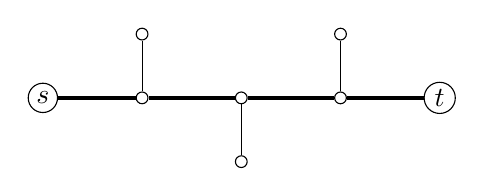
\begin{tikzpicture}[scale=0.9, every node/.style={circle, draw, inner sep=1.5pt}]
    \node (s) at (0,0) {$s$};
    \node (a) at (1.4,0) {};
    \node (b) at (2.8,0) {};
    \node (c) at (4.2,0) {};
    \node (t) at (5.6,0) {$t$};
    \node (x1) at (1.4,0.9) {};
    \node (x2) at (2.8,-0.9) {};
    \node (x3) at (4.2,0.9) {};
    \draw[very thick] (s)--(a)--(b)--(c)--(t);
    \draw (a)--(x1);
    \draw (b)--(x2);
    \draw (c)--(x3);
\end{tikzpicture}
\end{center}

有以下性质成立：

\begin{property}
    假设树无负权。任取一条直径 $(s,t)$，则对于任何一个点 $u$，$s,t$ 中至少有一个是距离 $u$ 最远的点之一。换句话说，距离一个点最远的点一定可以是直径的一个端点。
\end{property}
\begin{exercise}
    \begin{itemize}
        \item 说明在有负权时不成立。
        % 例如四点链 $a-b-c-d$ 的所有边权均为 $-1$，$(a,b)$ 是一条直径，但从 $d$ 出发的最远点是 $c$。
        \item 在边权和点权均非负，且距离 $d(u,v)$ 定义为路径上边权和加上 $u,v$ 两点的点权和时，证明该性质仍然成立。
    \end{itemize}
\end{exercise}
\begin{exercise}
    据此得到无负权树的直径的算法。
\end{exercise}
\begin{exercise}
    在有负权时，使用 DP 来计算直径。
\end{exercise}

下面的性质给出了连接两棵树后直径的变化。
\begin{property}
    假设树 $T_1$ 的一条直径是 $(s_1,t_1)$，树 $T_2$ 的一条直径是 $(s_2,t_2)$，并且边无负权。如果在两棵树中间加一条边得到一棵新树，那么新树中存在一条两个端点都在集合 $\{s_1,t_1,s_2,t_2\}$ 内的直径。
\end{property}
\begin{exercise}
    说明如何加边才能使得新树的直径最大/最小。
\end{exercise}
% \begin{solution}
%     若把 $x\in T_1$ 与 $y\in T_2$ 相连，则新直径长度为
%     $$
%         \max(D_1,D_2,\mathrm{ecc}_{T_1}(x)+c+\mathrm{ecc}_{T_2}(y)).
%     $$
%     因此最大化时连接两棵树各自的一个直径端点即可；最小化时连接两棵树的中心即可，此时答案为 $\max(D_1,D_2,R_1+c+R_2)$，其中 $R_i$ 是 $T_i$ 的半径。若题目只允许在原有顶点之间加边，则这里的中心和半径都取顶点意义下的最优值。
% \end{solution}
\begin{exercise}
    支持加边（保证任意时刻是森林）、查询某个连通块的直径。
\end{exercise}
% \begin{solution}
%     对每个连通块维护一组直径端点。合并两个连通块时，只需要在旧的四个端点之间枚举六对候选端点，取距离最大的一对作为新直径。
% \end{solution}
\begin{exercise}[P3596]
    给一棵树，对每条边，计算删除这条边然后再加一条新边后形成的树的直径可能的最大值和最小值。
\end{exercise}

对于边权为正的树，还有以下结论：
\begin{property}
    所有直径的中点（允许在边上）都相同。这个点称为树的中心（center），它最小化到树上所有点的最大距离。
\end{property}
\begin{remark}
    对于有零边的情况，可以把零边缩起来。
\end{remark}

\begin{exercise}[P1099/P2491]
    给定一棵非负权的树 $T$ 和一个常数 $s$，求一对点 $(u,v)$ 使得 $d(u,v)\le s$ 且 $\max_{x}\min_{y\in P_{uv}}d(x,y)$ 最小。也就是找到一条长度不超过 $s$ 的路径，使得到这条路径的最远距离最小。需要 $O(n)$。
\end{exercise}
\begin{exercise}[P3304]
    询问有多少条边满足所有的直径都经过它。
\end{exercise}

我们也可以定义一个点集内的直径。对于点集 $S$，定义 $S$ 内的直径为 $S$ 中距离最远的两点之间的距离。此时，有以下性质成立。
\begin{property}
    假设树无负权。任取点集 $S$ 内的一条直径 $(s,t)$，则对于树上的任何一个点 $u$，$s,t$ 中至少有一个是 $S$ 内距离 $u$ 最远的点之一。 
\end{property}
\begin{exercise}
    证明以下结论：任取点集 $S_1$ 内的一条直径 $(s_1,t_1)$ 和点集 $S_2$ 内的一条直径 $(s_2,t_2)$，则 $S_1\cup S_2$ 内存在一条两个端点都在 $\{s_1,t_1,s_2,t_2\}$ 内的直径。因此，点集内的直径是一种可以快速合并的分治信息。
\end{exercise}
\begin{exercise}
    多次询问 $S=[l,r]$ 内的直径。
\end{exercise}
\begin{exercise}
    给一棵树，维护一个点集 $S$，支持添加/删除点到 $S$ 中，查询 $S$ 内的直径。
\end{exercise}
\begin{remark}
    有负权时可以通过动态 DP 之类的方法做到 $O(\log n)$，参见 P4115。
\end{remark}
\begin{example}[CF1192B]
    修改边权，查询直径。保证边权非负。
\end{example}
\begin{remark}
    如果没有边权非负的保证，那么可以用静态 Top Tree 等方法做到 $O(\log n)$。
\end{remark}

\section{重心}

假设树 $T$ 带有非负的点权，且总点权大于零。定义一个点集 $S$ 的重量 $w(S)$ 为该点集内的点权和。树的重心（median/centroid）有以下两个等价定义：
\begin{itemize}
    \item 以重心 $u$ 为根时，$\max_{v\in \mathrm{son}_u}w(\mathrm{subtree}(v))$（最大的子树重量）最小。
    \item 以重心 $u$ 为根时，任何 $v\ne u$ 都满足 $w(\mathrm{subtree}(v)) \le w(T)/2$（每个子树的重量都不超过总重量的一半）。
\end{itemize}
\begin{remark}
    注意重心未必在直径上。
\end{remark}
直观上，重心可以这样取得：假设当前在点 $u$，考虑删掉 $u$ 形成的所有连通块，如果存在重量 $>w(T)/2$ 的那么就往这个连通块移动，否则 $u$ 本身就是重心。利用这个直观，我们可以得到以下性质：
\begin{property}
    \begin{itemize}
        \item 对一棵以 $r$ 为根的树，若 $r$ 不是重心，则存在唯一一个重量 $>w(T)/2$ 的儿子子树，并且所有重心都在这棵子树中。
        \item 假设 $u$ 是树的重心，并把树以 $u$ 为根。那么树除了 $u$ 之外的所有重心，恰好是满足 $w(\mathrm{subtree}(v))=w(T)/2$ 的点 $v$。在点权均为正的情况下，这样的点 $v$ 至多只有一个，故此时重心至多有两个且二者相邻。
    \end{itemize}
\end{property}

对于一棵以 $r$ 为根的有根树，在切换到以 $u$ 为根时，除了原本的子树外，还会产生一个“向上”的子树，这个子树的重量为 $w(T)-w(\mathrm{subtree}(u))$。可以据此判定一个点是否为树的重心。
\begin{exercise}[P5666]
    给一棵树，计算删除每条边后，形成的两个连通块中的所有重心的编号之和。
\end{exercise}

下面的性质将重心与距离联系在一起。
\begin{property}
    假设树的边权非负，距离定义为两点之间的路径的边权和。树的重心可以最小化所有点到它的距离之和，即 $\sum_v w_v \cdot d(v, u)$。
\end{property}
也可以据此定义点集内的重心：
\begin{definition}
    对于点集 $S$，定义 $S$ 内的重心为距离 $S$ 内所有点的距离之和最小的 $S$ 内的点，即 $\arg\min_{u \in S} \sum_{v \in S} w_v \cdot d(u, v)$。这里距离定义为两点之间路径上的边数（事实上任何非负边权导出的距离都可行）。
\end{definition}



下面的性质说明了连接两棵树后重心的变化情况。
\begin{property}
    假设树 $T_1,T_2$ 的点权均为正，且 $u_1,u_2$ 分别是它们的一个重心。如果在两棵树中间加一条边得到一棵新树，那么新树的所有重心都在 $u_1$ 和 $u_2$ 之间的链上。
\end{property}
\begin{example}[P4299]
    加边（保证任意时刻是森林），查询连通块重心。
\end{example}

下面的性质给出了重心与 DFS 序的联系。
\begin{property}
    DFS 序的带权中点定义为满足 $\sum_{i<k} w_{p_i} \le \frac{W}{2}$ 且 $\sum_{i>k}^n w_{p_i} \le \frac{W}{2}$ 的 $k$。这样的 $p_k$ 在深度最小的那个重心的子树内。
\end{property}
\begin{exercise}
    子树点权加/赋值，查询重心。
\end{exercise}
\begin{remark}
    后面我们学习链剖分之后还能支持链修改。
\end{remark}
\begin{exercise}
    查询 $S=[l,r]$ 内的重心。
\end{exercise}
\begin{solution}
    通过可持久化线段树/整体二分之类的方法求出 $S$ 在 DFS 序中的带权中点，然后从那个点向上跳到最后一个子树内有至多 $w(S)/2$ 重量的点即可。
\end{solution}